\documentclass{article}
%\usepackage{geometry}
%\geometry{top = 1in, bottom = 1in, left = 1in, right = 1in}
\usepackage[top = 0.7in, bottom = 0.7in, left = 0.7in, right = 0.7in]{geometry}
\usepackage{amsmath,amssymb,amsthm,mathrsfs}
\usepackage{graphicx}
\usepackage{bm}
\usepackage{float}
\usepackage[font=footnotesize,labelfont=bf]{caption}
\usepackage{movie15}
\usepackage{hyperref}

\usepackage{fancyhdr}
\pagestyle{fancy}
\rhead{\footnotesize {07/27/2012 ; MESA version 4161} }
\chead{\footnotesize {Authors: Jared Brooks, Lars Bildsten, Bill Paxton} }
\lhead{\footnotesize {mesa/star/test\_suite/ns\_h} }

\begin{document}
	
	\begin{center}
		\begin{Large}
		       \textbf{NS H}\\
		\end{Large}
	\end{center}
	
        This test is to show a 1.4 $\Msun$ neutron star undergoing a thermonuclear instability.  To check if this test ran successfully, the luminosity range from the run is checked against accepted values.  If the luminosity did not dip too low and the maximum luminosity exceeds a certain threshold, the terminal output at the end of the run should read \texttt{``all values are within tolerance''}.\\

        \underline{Note}: \texttt{MESA} is not computing the core of the neutron star, consider the ``core'' of the model the bottom of the envelope.\\

        This test case creates the envelope of a neutron star, and slowly accretes material at a rate of $1.7\times10^{-11} \Msun$/yr (\texttt{mass\_change = 1.7d-11}).\\

        \noindent Accreted Material composition (mass fractions):
        \begin{itemize}
                \item $^1$H: 0.72
                \item $^4$He: 0.26
        \end{itemize}

        This burst has a clear start and finish, and only lasts about 13 hours, as shown by the luminosity (figure \ref{fig:1}) and effective temperature (figure \ref{fig:2}) plots below.

        \begin{figure}[H]
                \begin{minipage}[b]{0.5\linewidth}
		       \centering
		       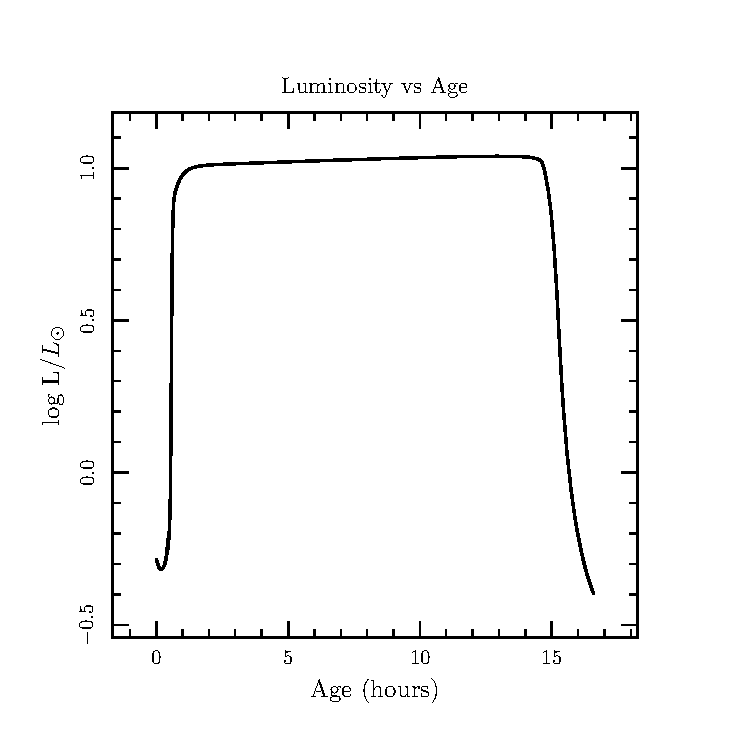
\includegraphics[width = 3.8in]{/Users/jaredbrooks/ns_h/plots_out/Luminosity_vs_Age.pdf}
		       \caption{Luminosity plot shows burst period}
		       \label{fig:1}
                \end{minipage}
                \hspace{0cm}
                \begin{minipage}[b]{0.5\linewidth}
                       \centering
                       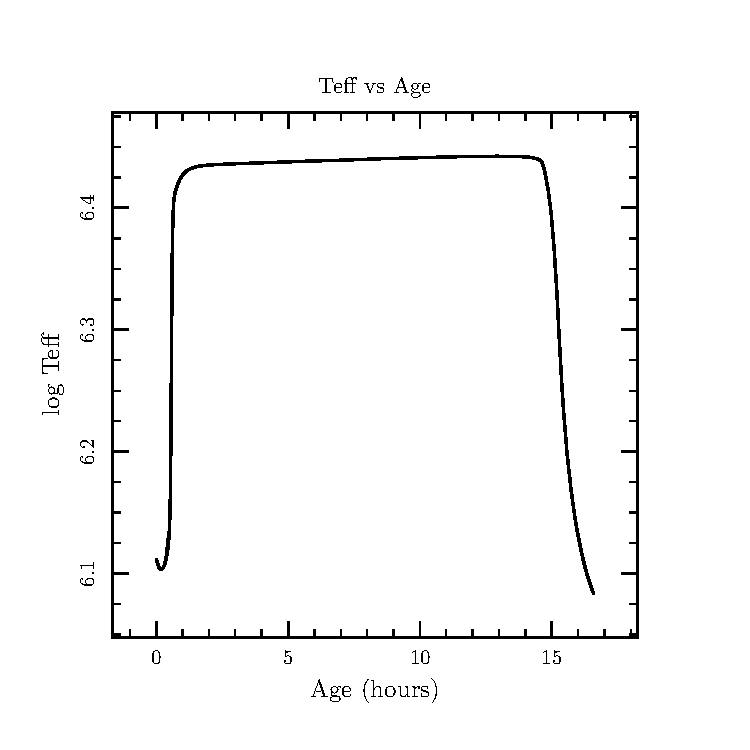
\includegraphics[width = 3.8in]{/Users/jaredbrooks/ns_h/plots_out/Teff_vs_Age.pdf}
                       \caption{Effective temperature shows burst period}
                       \label{fig:2}
                \end{minipage}
	\end{figure}

        \pagebreak

        The nuclear burning during the burst, characterized by the burning rate profile to the left (figure \ref{fig:3}), is dominated by the CNO cycle.  Therefore, this burst comes to an end when the majority of hydrogen is used up, shown in the plot to the right (figure \ref{fig:4}).

        \begin{figure}[H]
                \begin{minipage}[b]{0.5\linewidth}
                       \centering
                       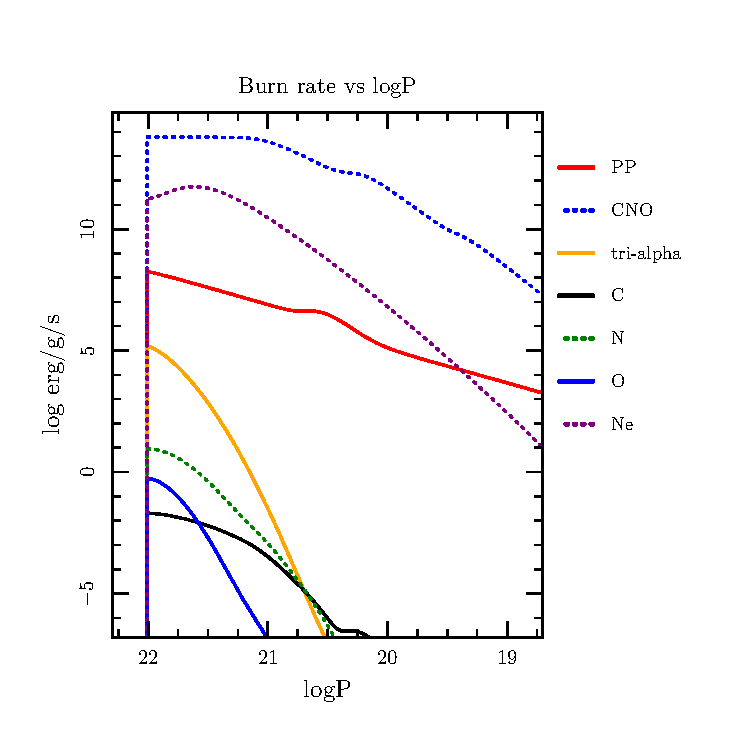
\includegraphics[width = 3.8in]{/Users/jaredbrooks/ns_h/plots_out/Burnrate_vs_logP_finish.pdf}
                       \caption{Burning rate profile during the burst, dominated by CNO}
                       \label{fig:3}
                \end{minipage}
                \hspace{0cm}
                \begin{minipage}[b]{0.5\linewidth}
                       \centering
                       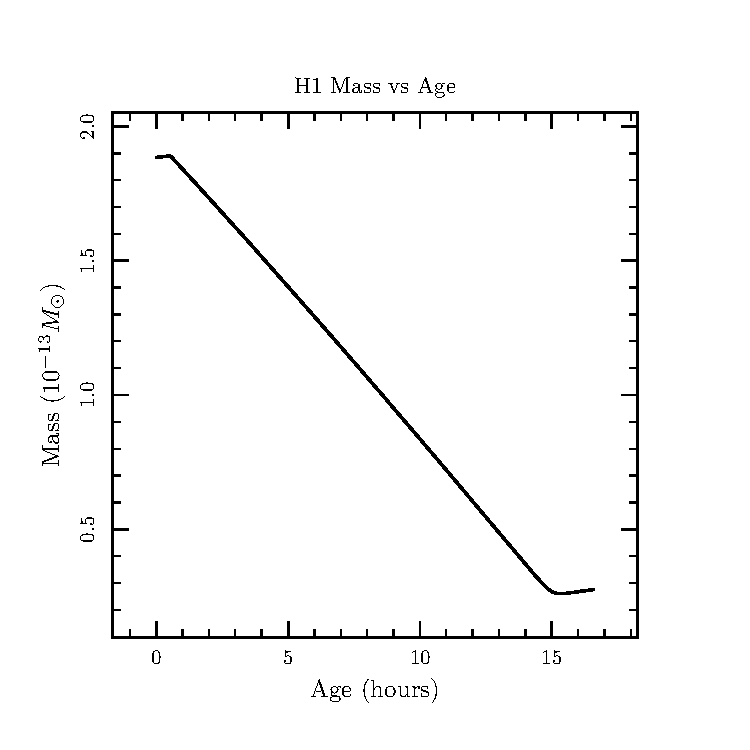
\includegraphics[width = 3.8in]{/Users/jaredbrooks/ns_h/plots_out/H1_Mass_vs_Age.pdf}
                       \caption{Hydrogen mass plot shows most of hydrogen used up by end of burst}
                       \label{fig:4}
                \end{minipage}
        \end{figure}

        \pagebreak

        Below is a video showing changes in abundances of elements plotted against logP.  The number at the top-right is the model number.  Click the figure to begin the video, double click to replay (must be using adobe reader to view movie).  Below that are two abundance profiles, at the start of the burst to the left (figure \ref{fig:5}) and after the burst to the right (figure \ref{fig:6}), to show what elements were consumed and what elements were produced during the burst.  (Note: The Ne20 shown here actually represents Ne22, this is because \texttt{MESA} is using a simplified nuclear reaction network.)

        \begin{figure}[H]
          \includemovie[poster,text={\small(Loading Video...)}]{18cm}{15cm}{abun.mp4}
        \end{figure}


        \begin{figure}[H]
                \begin{minipage}[b]{0.5\linewidth}
                       \centering
                       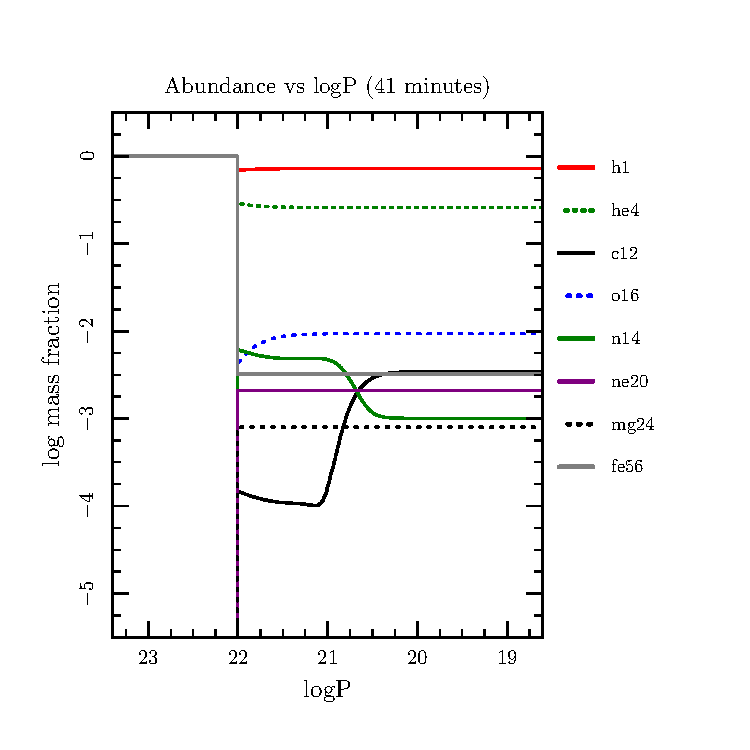
\includegraphics[width = 3.8in]{/Users/jaredbrooks/ns_h/plots_out/Abundance_vs_logP_2.pdf}
                       \caption{Abundance profile at the start of the burst}
                       \label{fig:5}
                \end{minipage}
                \hspace{0cm}
                \begin{minipage}[b]{0.5\linewidth}
                       \centering
                       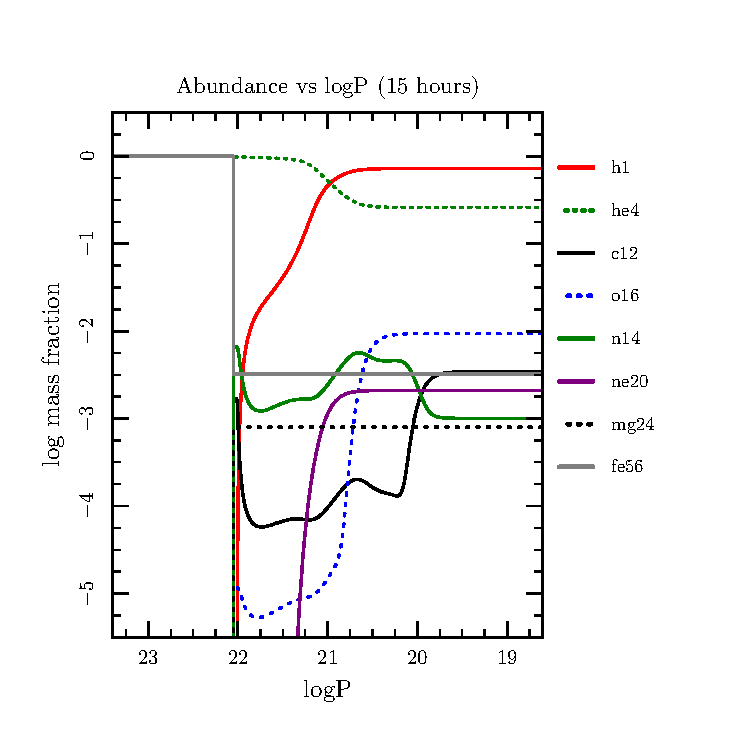
\includegraphics[width = 3.8in]{/Users/jaredbrooks/ns_h/plots_out/Abundance_vs_logP_4.pdf}
                       \caption{Abundance profile after the burst}
                       \label{fig:6}
                \end{minipage}
        \end{figure}

        \pagebreak

        This final plot (figure \ref{fig:7}) is meant to show a few internal \texttt{MESA} variables, such as the size of the time-step, the number of zones, and the number of retries against the model number in order to give some understanding of how hard \texttt{MESA} is working throughout the run and where some areas of problems/interest might be.

        \begin{figure}[H]
                \centering
                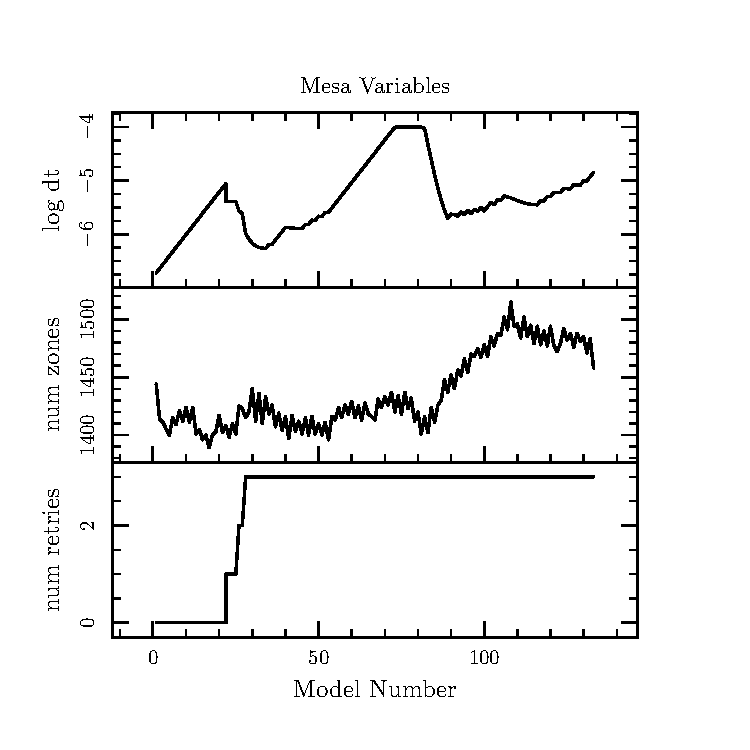
\includegraphics[width = 5in]{/Users/jaredbrooks/ns_h/plots_out/Mesa_Variables.pdf}
                \caption{\texttt{MESA} variables plotted against model number show how hard \texttt{MESA} is working}
                \label{fig:7}
        \end{figure}

\end{document}
